\documentclass{article}
 
\usepackage{amsmath}
\usepackage{amssymb}
\usepackage{graphicx}
\usepackage{verbatim}
\usepackage{enumerate}
\usepackage[utf8]{inputenc}
\newcommand{\beq}{\begin{equation}}
\newcommand{\eeq}{\end{equation}}
%\verbatiminput{verb.txt}
\begin{document}
\title{Compulsory assignment\\Deadline: 26th March 2014}
\author{Shafa Aria}
\maketitle
\begin{enumerate}[I]
\item For part one we will study the following distribution $X = \sum_{i=1}^N x_i$ where the random increments $x_i$ are distributed by various distributions.\\

To start off, we set $x_0 = 1$ and update $x_{i+1}=-x_i$ with probability $p$ and $x_{i+1} = x_i$ with probability $1-p$. We will first run the simulation for $N=1000$ with $10^5$ realisations and find $\langle X^2\rangle$. 
\begin{verbatim}
For p = 0.500 we get <X^2> = 999.70
For p = 0.100 we get <X^2> = 8914.41
For p = 0.010 we get <X^2> = 94960.90
\end{verbatim}
As is expected the lower value we assign to $p$ the lower will the chances be that our random walk will drift towards the negative direction.

For the next step we would like to plot the variance $\log_{10}(\langle\Delta X^2\rangle)$ as a function of $\log_{10}(i)$ and try to identify the linear portions of the graphs.\\
\hspace{-4cm}
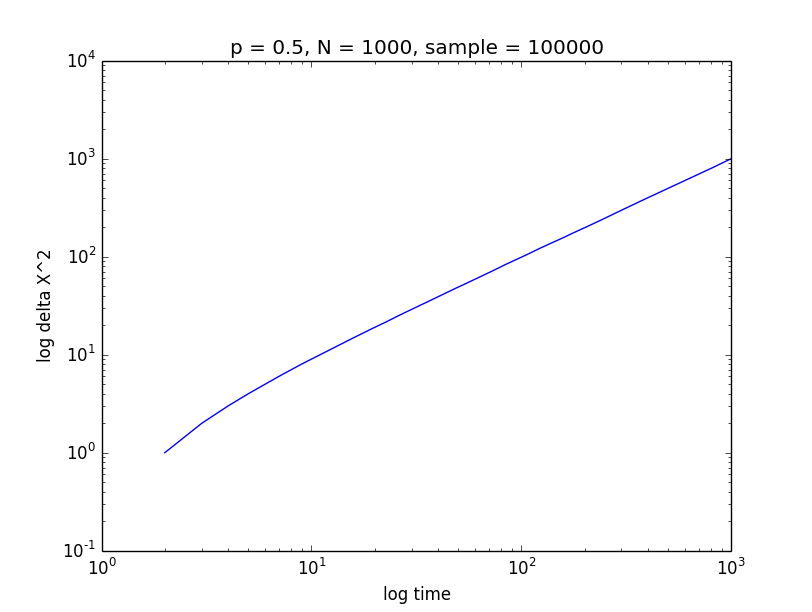
\includegraphics[scale=0.3]{05log.png}
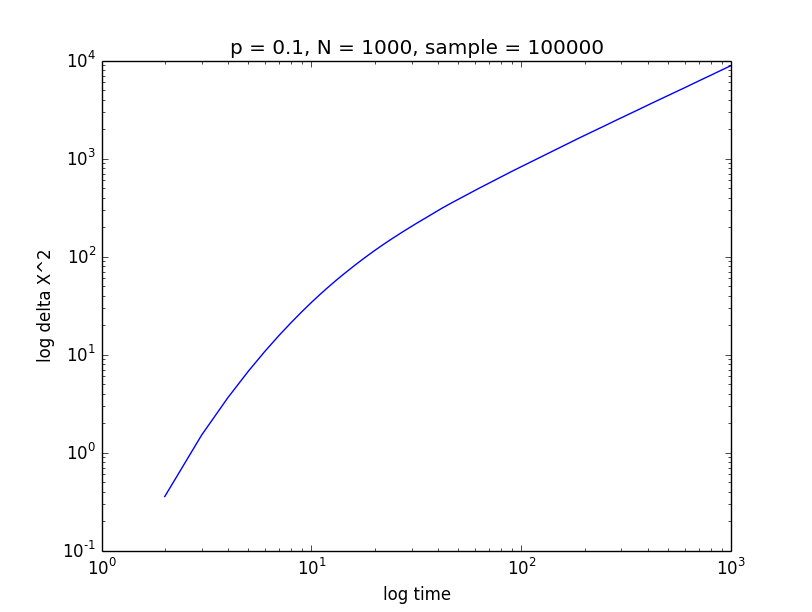
\includegraphics[scale=0.3]{01log.png}
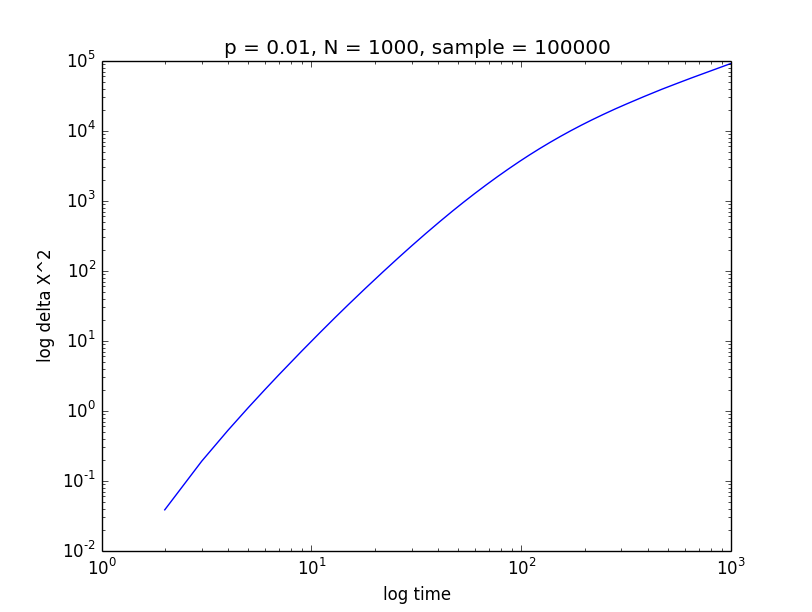
\includegraphics[scale=0.3]{001log.png}
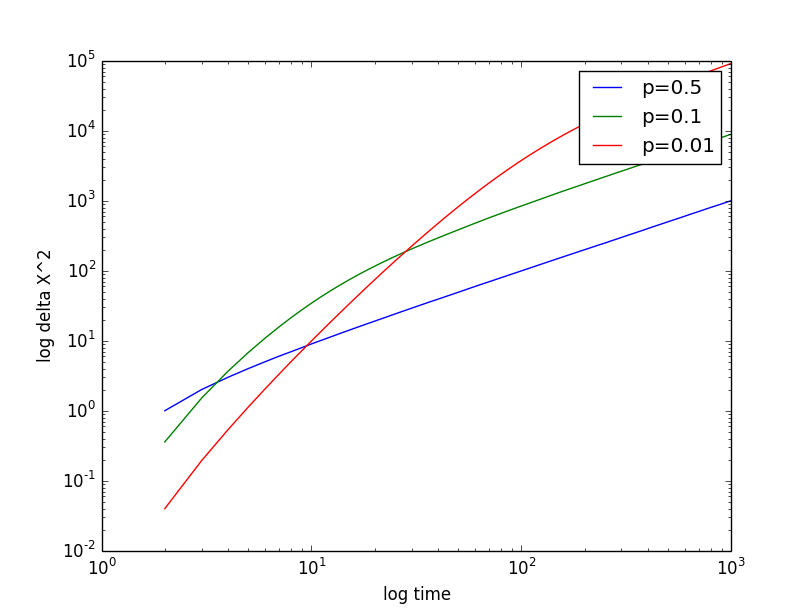
\includegraphics[scale=0.3]{alog.png}\\
As we would have expected for $p=0.5$ it is more or less constant. From the looks of it we could perhaps say that the lower the $p$ value the further uninterrupted do the particles propagate thereby creating lower $\langle X \rangle$, but higher $\langle X^2 \rangle$.\\

The probability $P_n(S)$, which is the probability to find the particle at position $x=Sa$ at time $t=N\tau$, satisfies the stochastic equation $P_{N+1}(S) = pP_N(S-1) + qP_N(S+1)$. Here, $p$ is the probability for a step to the right and $q=1-p$ is the probability for a step to the left, $\tau$ is the time for a single step length $a$ and $S$ is the net displacement.

We will confine ourselves to the case where there is an equal probability for either direction i.e. $q=p=0.5$. In this case the above equation can be written as 
\[P_{N+1}(S)=\frac{1}{2}P_{N}(S-1)+\frac{1}{2}P_{N}(S+1)\]
Subtracting $P_{N}(S)$ on both sides
\[P_{N+1}(S)-P_{N}(S)=\frac{1}{2}\left(P_{N}(S-1)+P_{N}(S+1)-2P_{N}(S)\right)\]
When the number $N$ of steps in the walk becomes very large, we can assume that each step is very small of length $a$ and thus the differences become differentials.
The LHS can be written as $\tau \frac{\partial P}{\partial t}$ and the RHS $\frac{1}{2}a^2 \frac{\partial^2 P}{\partial x^2}$. We can then write this as 
\[\frac{\partial P}{\partial x}=\frac{a^2}{2\tau} \frac{\partial^2 P}{\partial x^2}\]
or
\[\frac{\partial P}{\partial x}=D \frac{\partial^2 P}{\partial x^2}\]
where $D=\frac{a^2}{2\tau}$ is the diffusion coefficient. Solving this diffusion equation for all time $t$ with boundary conditions $P(\pm\infty,t)=0$ and the initial condition $P(x,0) = \delta(x)$ i.e we have a delta peak at the origin. The solution is then
\[P(x,t) = \frac{1}{\sqrt{2\pi\sigma^2}}e^{-\frac{x^2}{2\sigma^2}}\]
where $\sigma^2 = 2Dt$ as we shall see later on. The mean square displacement in 1D is then given by 
\begin{align*}  
\langle x^2 \rangle &= \int_{-\infty}^{\infty} x^2P(x)\mathrm{d}x\\
 &= \frac{1}{\sqrt{4\pi Dt}}\int_{-\infty}^{\infty} x^2 e^{-\frac{x^2}{4Dt}}\mathrm{d}x\\
 &= \frac{1}{\sqrt{4\pi Dt}}\int_{-\infty}^{\infty} x^2 e^{-\frac{x^2}{4Dt}}\mathrm{d}x\\
\end{align*}
We note that the function we are trying to integrate is an even function and thus symmetric. We omit the lower integration limit and rewrite the equation as
\[\langle x^2 \rangle = \frac{2}{\sqrt{4\pi Dt}}\int_{0}^{\infty} x^2 e^{-\frac{x^2}{4Dt}}\mathrm{d}x\]
or as
\[\langle x^2 \rangle = \frac{2}{\sqrt{4\pi Dt}}\int_{0}^{\infty} x^k e^{-\lambda x^2} \mathrm{d}x\]
where $k=2$ and $\lambda = \frac{1}{4Dt}$. This familiar integral can be looked up in Rottman's formula book or by using \texttt{sympy}. 
\[\langle x^2 \rangle = \frac{2}{\sqrt{4\pi Dt}}\frac{1}{2}\left(\frac{1}{4Dt}\right)^{-\frac{3}{2}}\Gamma\left(\frac{3}{2}\right) \] 
The Gamma function is given by $\Gamma\left(\frac{n}{2}\right) = \sqrt{\pi}\frac{(n-2)!!}{2^{(n-1)/2}}$ which by setting in $n=3$ gives us
\[\langle x^2 \rangle = \frac{1}{\sqrt{4\pi Dt}}\sqrt{(4Dt)^3}\frac{\sqrt\pi}{2} = \frac{1}{2}\sqrt{\frac{(4Dt)^3 \pi}{4\pi Dt}}\]
\[\langle x^2 \rangle = 2Dt\]
We can easily find the $D$ value by computation:
\texttt{0.502407069735}
as expected $D\approx 0.5$\\

Physically we would assume $p$ to be associated to a particles willingness to change direction. Another way to look at it is to imagine a particle propagating in one direction, as long as it does not collide with another particle it will keep propagating in that direction. If, on the other hand, it collides with another particle, it will change its direction. For lower $p$ values we can imagine us the system being in an ideal gas state where no particle collision is taking place and as we increase the $p$ values it will result in lower variance.

Say we have a low $p$ value and the particle starts off in one direction then it is less likely to change to the other direction as opposed to higher values which will yield higher collision rates and thus change in direction (for $p=0.5$ that would be every other step).

We will try to plot the $X_N$ in a histogram\\
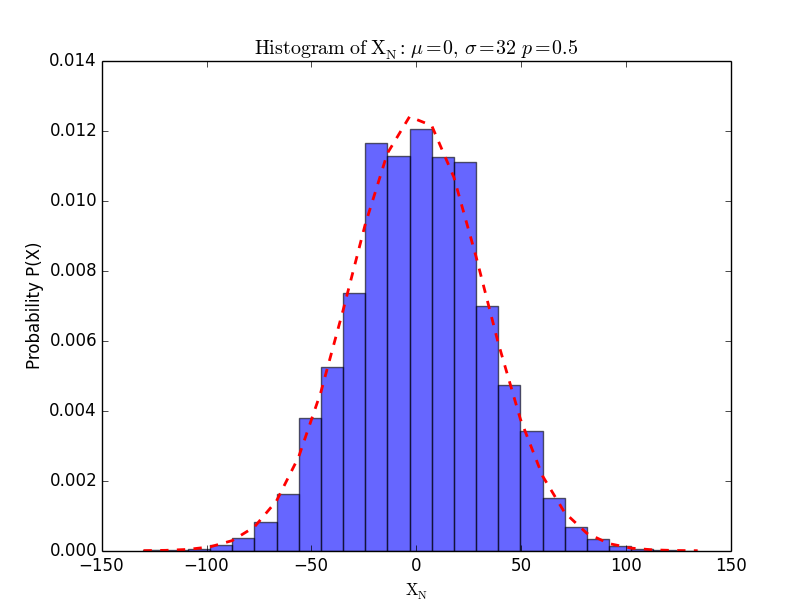
\includegraphics[scale=0.3]{hist05.png}
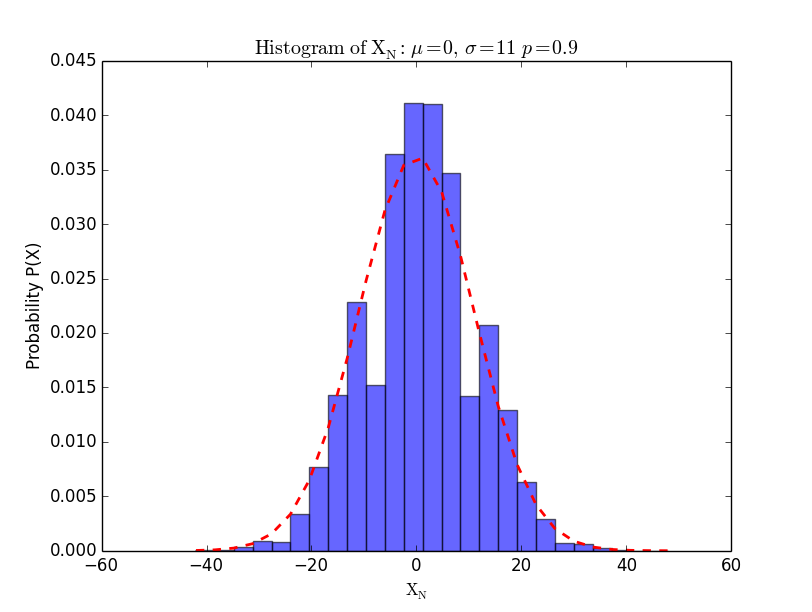
\includegraphics[scale=0.3]{hist09.png}
\begin{center}
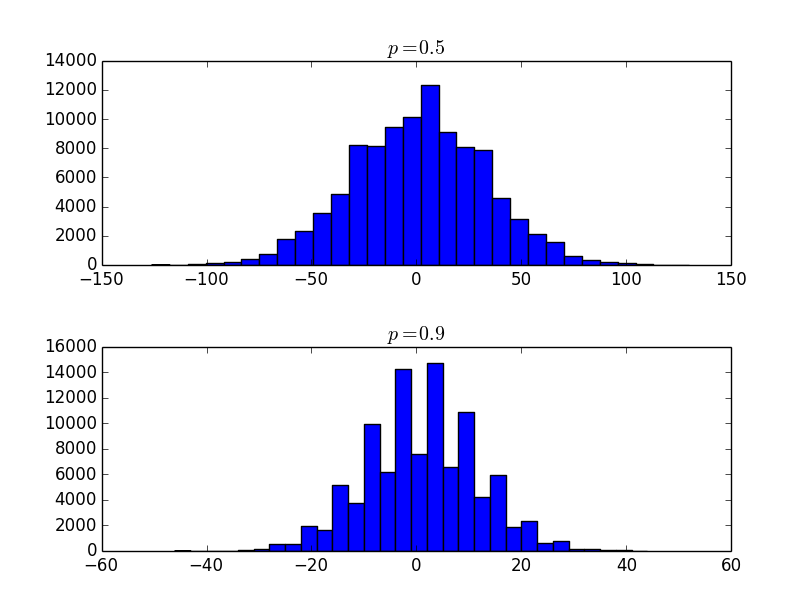
\includegraphics[scale=0.3]{histo.png}  
\end{center}
Using the obtained values from the histogram above we can use it in our $P(X)$ function to plot $X^2$ against $\log(P(X))$. \\
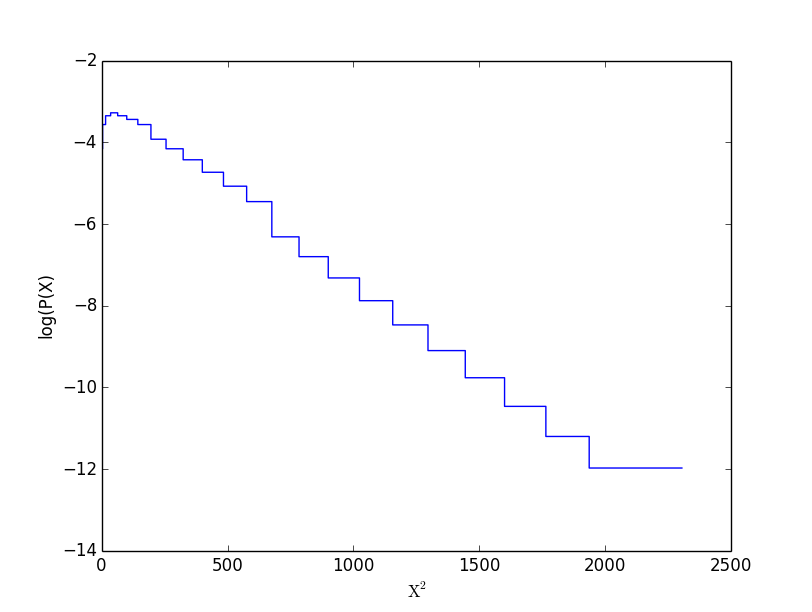
\includegraphics[scale=0.3]{lastone.png}  
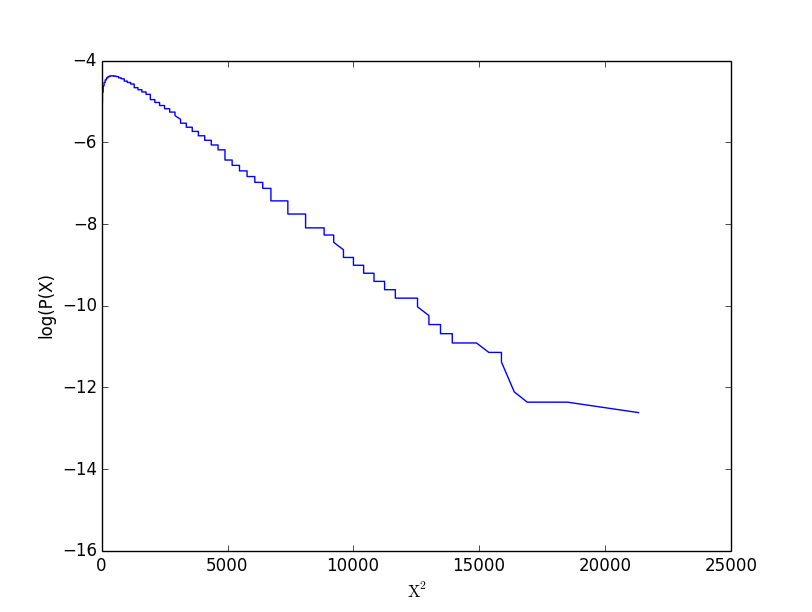
\includegraphics[scale=0.3]{lastone1.png}  



From the lecture notes we have that $\langle X^2 \rangle = N\sigma^2$ and we know from previously that for $p=0.5$, $\langle X^2 \rangle = 2Dt$, where $D=a^2/(2Nt)$
\newpage
\item
First let us consider the following equation 
\[ |\mathbf{E}_0|=\cos(\mathbf{k}\cdot\mathbf{r} - \omega t) \]
Where plugging into the wave equation yields $\omega^2 = k^2 c^2$ and from Maxwell's equations we have $\nabla \cdot \mathbf{E} = 0$ which gives $\mathbf{k} \cdot \mathbf{E}_0$. The vector $\mathbf{E}$ is therefore orthogonal to the propagation vector $\mathbf{k}$. Furthermore we have assumed periodic boundary condition, in two dimension this is\\ 
\[k_xL = 2\pi n_x, \hspace{2cm} n_x = 0, \pm1, \pm2...\]
\[k_yL = 2\pi n_y, \hspace{2cm} n_y = 0, \pm1, \pm2...\]
We see compared to fixed boundary conditions $\mathbf{k}$ is separated by twice as large interval, but $n_{x,y}$ can be both positive and negative and each giving independent solutions.\\

The average energy of the oscillator is given by (5.38)
\[\langle \epsilon_\mathbf{k} \rangle = (kT)^2 \frac{\partial \log Z}{\partial kT}= \frac{\hbar \omega}{e^{\hbar \omega /kT} - 1} \] 
Where $Z$ would be the partition function. Furthermore we have the given spectral density as 
\[ \mathcal{E}(\omega,T) = \frac{\omega^2}{\pi^2 c^3}\frac{\hbar \omega}{e^{\hbar \omega /kT} - 1} \] To find the internal energy we shall take the integral of the above equation with respect to the frequency. 
\begin{align*}
U(T) &= \int_0^\infty \mathrm{d}\omega\mathcal{E}(\omega, T)V \\
&= V \int_0^\infty \mathrm{d}\omega \frac{\omega^3}{\pi^2 c^3}\frac{\hbar}{e^{\hbar \omega /kT} - 1}\\
\end{align*}
By setting $x= \frac{\hbar \omega}{kT}$ we get the following form:
\begin{align*}
&= V \frac{(kT)^4}{\pi^2 c^3 \hbar^3} \int_0^\infty \mathrm{d}x \frac{x}{e^{x} - 1}\\
&= V \frac{(kT)^4}{\pi^2 c^3 \hbar^3} \frac{\pi^4}{15}\\
\end{align*}
Where we have looked up the integral, yielding the final result:
\[ U(T) = \left( \frac{\pi^2 k^4}{15 c^3 \hbar^3}\right) VT^4\]
The heat capacity is given by $C_v = \left(\frac{\partial U}{\partial T}\right )_V$. Performing the differentiation yields:
\[ C_V = \left( \frac{4\pi^2 k^4}{15 c^3 \hbar^3}\right) VT^3\]
\end{enumerate}
\section{Code}
The code is available at github:
\texttt{www.github.com/Ace-}
\end{document}
